This chapter will look at the performance of the Simulator as a whole as well as the performance of the ML-Agents. As this is only a prototype the performance is not the most important aspect. The chapter will also look at the experiments conducted.

The results studied in this chapter would be from individual features of the simulator rather than the simulator as a whole. The features that were added to the simulator were mentioned in the implementation chapter (Chapter~\ref{implementation}).

% As this is an implementation project, most of the testing was discussed in the Implemenation section.  
\section{Simulator Performance}
This section will look at what experiments were conducted on the simulator to evaluate its performance. It is worth noting that as this is a prototype, the efficiency of the implementation is not important. 

A lot of testing is also done manually. Features that are not done through the API such as camera control and vehicle handling was therefore not tested using scripts. 

\subsection{Basic Features - API}
The python client folder on GitHub\footnote{\url{https://github.com/tobhil98/MastersProject-AirSim/tree/master/PythonClient}} contains a variety of scripts that could be used to test the simulator. There are no unit tests however as  Figure~\ref{08:PythonLogic} shows how a test can be implemented. The green boxes indicate actions that have to be done by the client, and the red boxes indicate API calls. 

Inside the car folder the car\_stress\_test is very similar to this figure. Here a car will spawn and drive in a direction for a second return the fetch internal car state, stop, and then drive in another direction for a second. The internal car state will contain information such as the position and speed of the vehicle. This test shows that the APIs work and that the vehicle asset is available. 

Another test car\_test\_many. This has been used to test how many entities the simulator can handle. If the cameras are not enabled the simulator can handle over 100 entities, however, as can be observed from Figure~\ref{06:frameRates} not many the simulator suffers quite quickly when there are several cameras in the scene. 

\begin{figure}[H]
\centering
    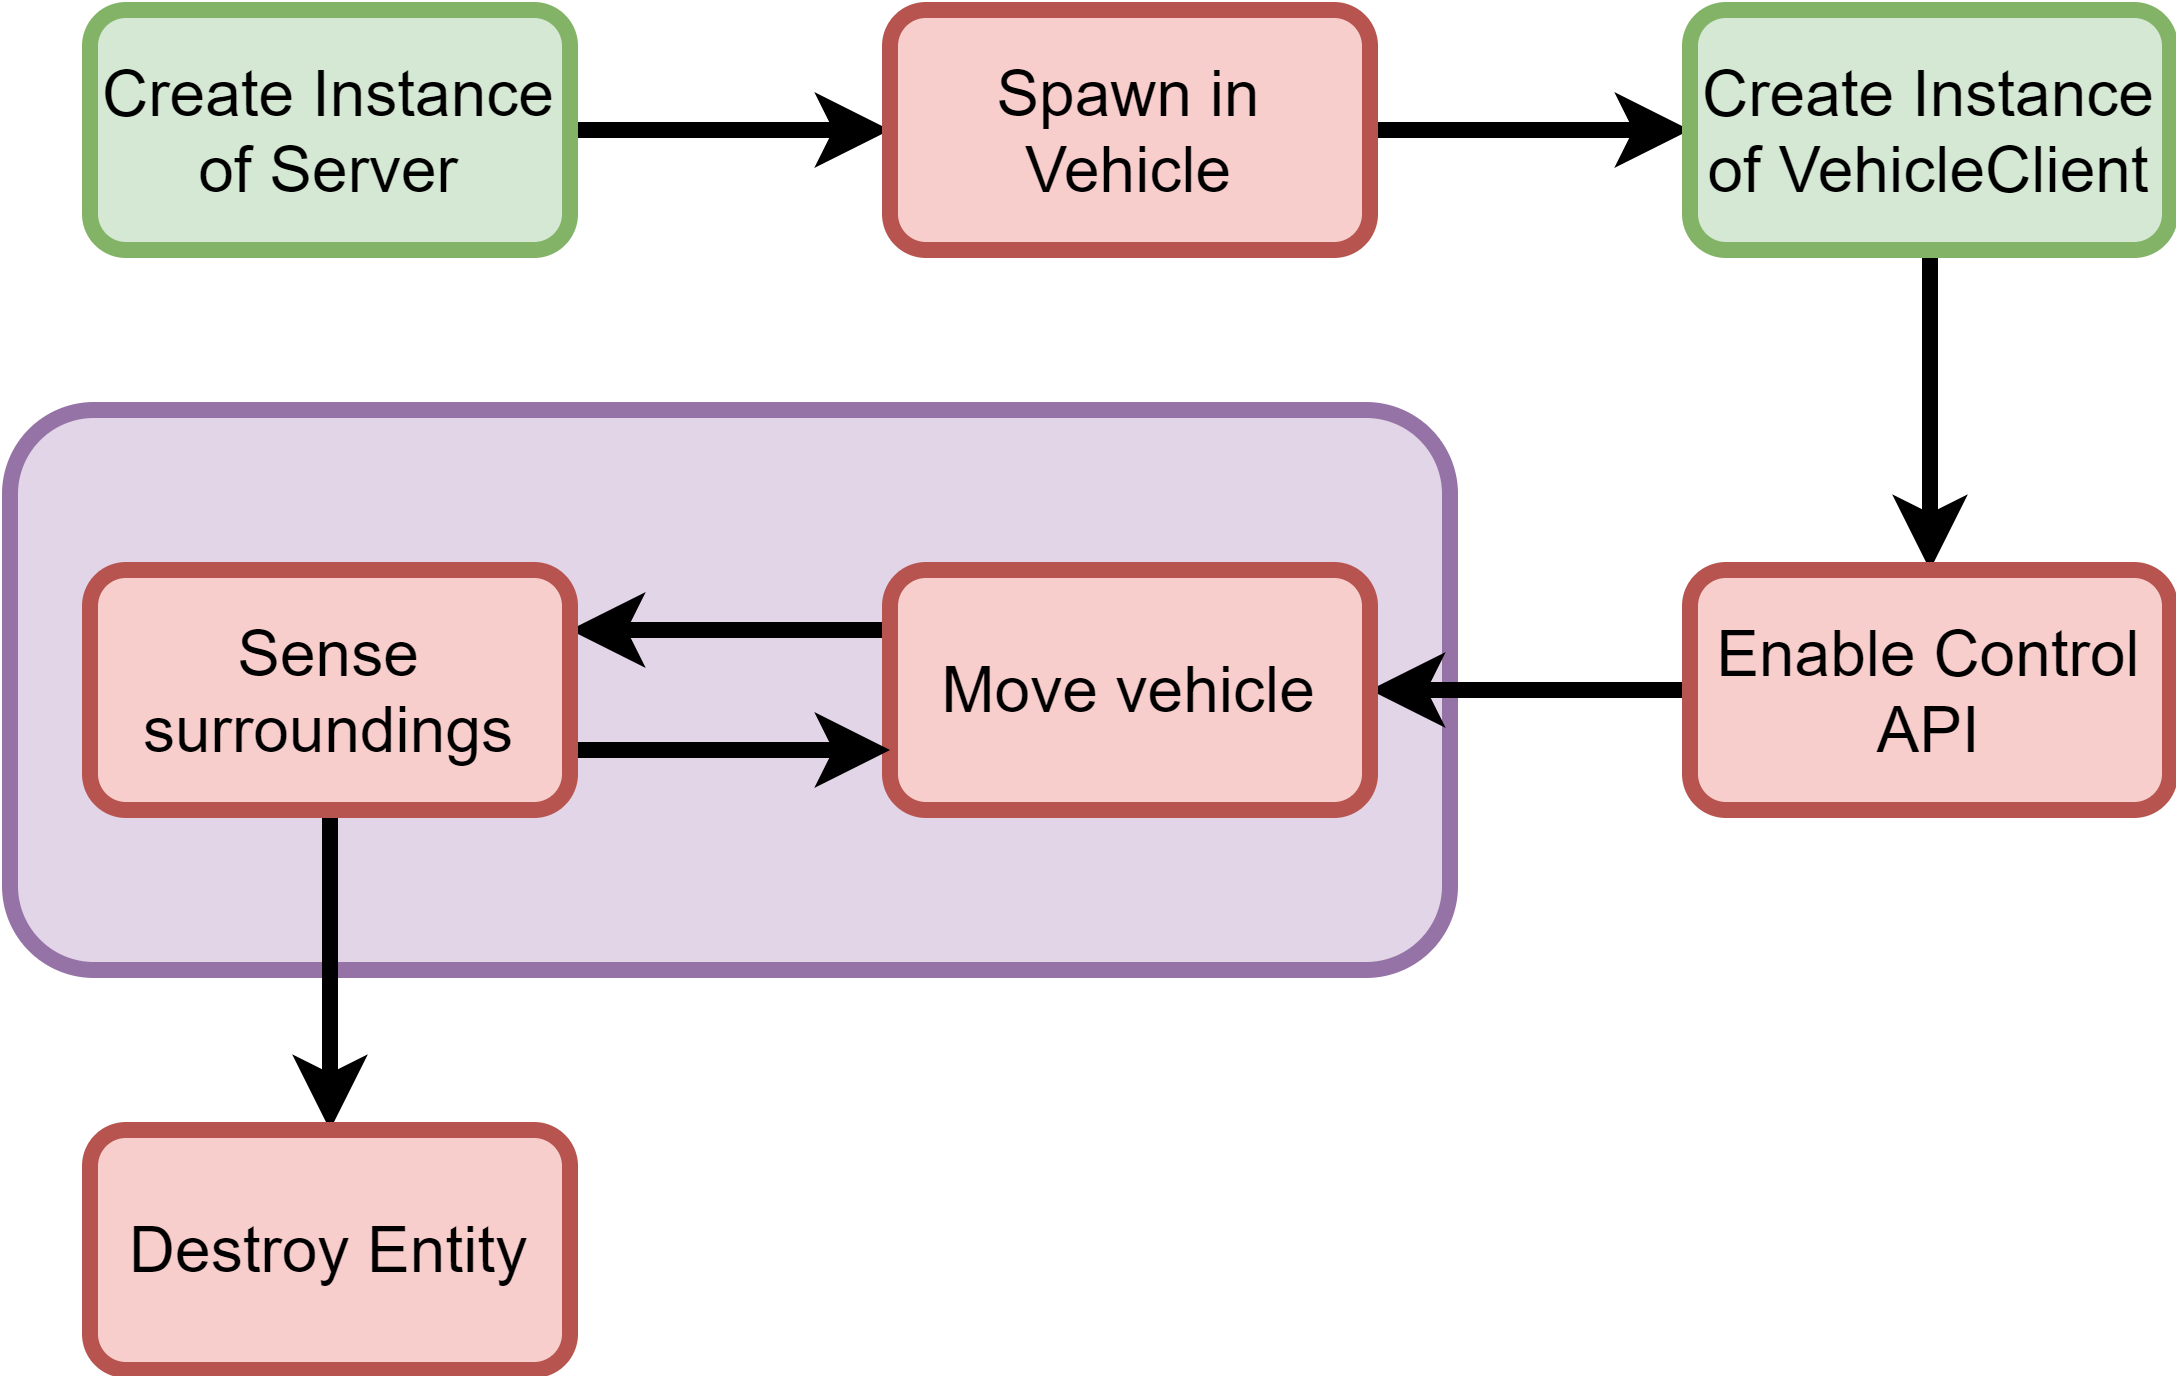
\includegraphics[width=0.5\textwidth]{08_Results/PythonLogicCycle.png}
    \caption[Python Logic Flow]{Red boxes indicates API calls, whilst green indicate processing in Python. The purple box is to indicate the functions happening when the simulator is running and the vehicles are moving around.} \label{08:PythonLogic}
\end{figure}




\subsection{Testing the video feed}
Figure~\ref{06:frameRates} illustrates the decreasing tick rate of the simulator as the number of cameras increases.  As was mentioned in Section~\ref{06:VideoFeed}, this was introduced to counter the slow response time. A key point to note here is that this diagram looks at the tick speed of the game, not just the frame rate. Cinemas typically show their films at 25 frames per second, and as can be observed from the figure, with around 75 cameras the simulator can run at around 20 ticks per second if the frame rendering ratio is 1:6. Even though the simulator looks smooth, it would be running much slower than usual, as the normal speed would be 120 ticks per second. The simulator is therefore running at roughly 16\% speed, making moving around and driving a vehicle difficult. Currently, this is a limitation of Unity. Unity does not allow threading of monobehavior which contains all the functions that can interact with the simulator. (See appendix~Figure~\ref{A:MonobehaviorFlow})

\begin{figure}[H]
    \centering
    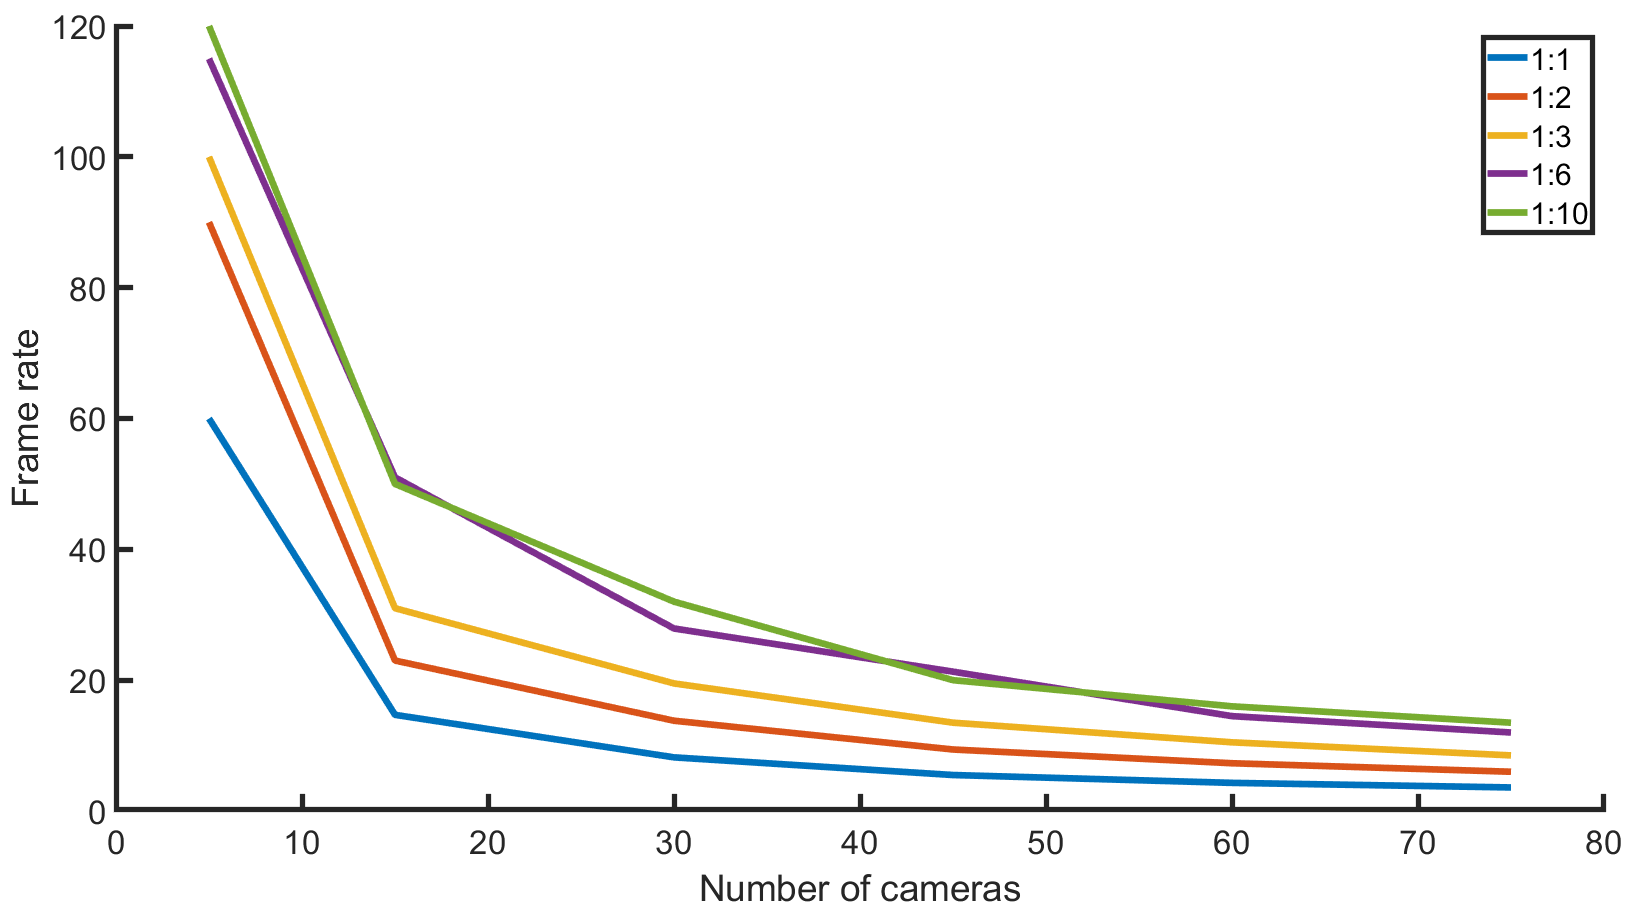
\includegraphics[width=0.85\textwidth]{06_Implementation/00_AirSim/Diagrams/frameRates.png}
    \caption[AirSim tick rates]{As the number of cameras are added to the scene the simulator frame rate decreases. By not rendering every camera on every frame the simulator frame rate increases. Each line represents a ratio for how often the camera renders, i.e. 1:2 means the camera frame is rendered every other game update.} \label{06:frameRates}
\end{figure}


\subsection{Unity Profiler}
This is just a quick overview of the profiling tool in Unity. This can be used to see how long a computation takes or how much resources it uses. Even though it is a bit small, most of the time whilst running is spent in the fixed update block (Figure~\ref{08:profiler}). 
\begin{figure}[H]
    \centering
    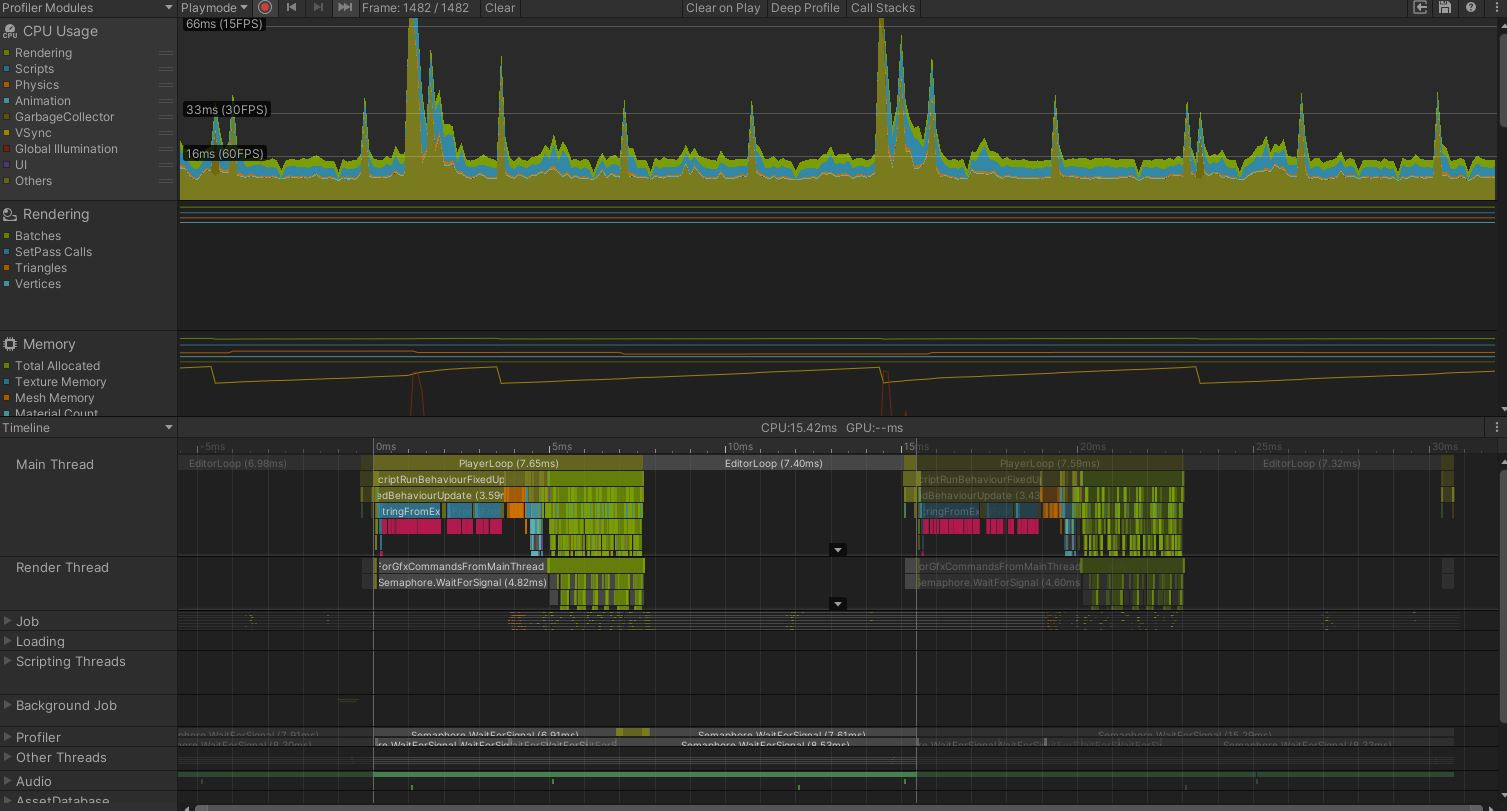
\includegraphics[width=1\textwidth]{08_Results/UnityProfiler.JPG}
    \caption[Unity Profiler]{The Unity profiler allows the developer to see what the in the game engine how computationally a task is.} \label{08:profiler}
\end{figure}


\section{ML-Agents Performance} \label{MLPreformance}
This section will look at the performance of autonomous vehicles as well as the tuning process. This section will be split into two parts. The first part is an environment where the vehicle could drive around by itself. The second part will look at the vehicles using collaboration learning. 

Along with ML-Agent TensorBoard is imported. TensorBoard is a visual toolkit that allows displaying matrices such as the environment and loss from the learning.  

\subsection{Training using PPO}
As mentioned in the implementation section, the two options that could be used for this section were PPO or SAC. As SAC is designed to run slower and make more complex decisions PPO would be the one to use. 

To avoid too many plots only the most interesting runs have been extracted. It is also worth noting that the vehicle simulation is more of a proof of concept to prove what is possible with the simulator rather than a perfect solution. 

\subsubsection{Discrete vs Continuous}

Figure~\ref{08:DiscreteVsCont} shows the cumulative reward per episode and episode length. It is clear that the light blue line reaches the reward target quickly whilst the other line stays at a negative value. This is using the simple map where the vehicles only had to drive in circles until it timed out. The hyperparameters are the same with the only difference being that the light blue model is producing discrete output values and the dark blue is producing continuous. 

It can also be observed that there is a small dip at around 1M steps where after that the dark blue episode length started increasing. This was most likely caused by the vehicle not moving and the penalty received was the standard one received per time step. 

It is quite clear from this plot that using discrete values worked better than continuous. 

\begin{figure}[H]
    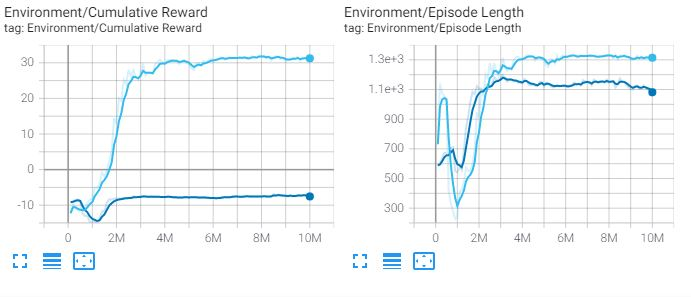
\includegraphics[width=1\textwidth]{08_Results/ML-agent results/DiscreteVContinous1.JPG}
    \caption[Discrete vs Continuous]{The light blue line indicates a discrete model output, whilst the dark blue shows the continuous. The other hyperparameters are the same in both runs.} \label{08:DiscreteVsCont}
\end{figure}


\subsubsection{Model depth}
This part will look at the two alternatives to the network structure. ML-Agents recommend having between 2 to 3 hidden layers in the model. Figure~\ref{08:DiscSimp} shows the cumulative reward and episode length on the simple map. The performance of the two models is very similar. However, training the deeper network took 30\% longer time than when training the network with 2 layers. On the more complex map, the difference becomes more noteworthy. The wider shallower layer quickly adapts to reach the higher rewards. This could have something to do with the number of inputs. As it is quite large, having a shallower network distinguishes this better. 

\begin{figure}[h]
    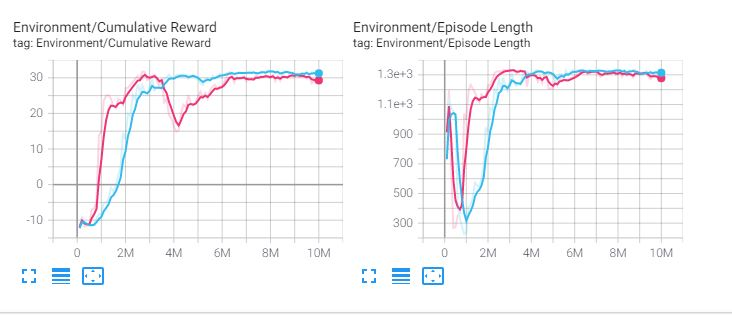
\includegraphics[width=1\textwidth]{08_Results/ML-agent results/NetworksDiscrete.JPG}
    \caption[Discrete network - Simple map]{Pink line indicates model with 2 hidden layers and 128 neurons in each. Blue line indicates 3 hidden layers with 64 neurons in each. Same performance after not many iterations, but the deeper network took 30\% longer.} \label{08:DiscSimp}
\end{figure}
\begin{figure}[h]
    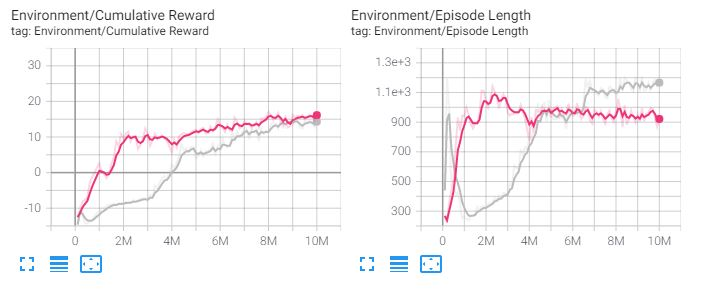
\includegraphics[width=1\textwidth]{08_Results/ML-agent results/NetworksDiscreteSimple.JPG}
    \caption[Discrete network - Complex map]{Pink line indicates model with 2 hidden layers and 256 neurons in each. Grey line indicates 3 hidden layers with 64 neurons in each.} \label{08:DiscAdv}
\end{figure}

\subsubsection{Other parameters tuned}
There are several other parameters to tune. These include the number of network design of the GAIL model, learning rate, and policy variables. However, the models did not improve when these were tweaked. 
\FloatBarrier
\pagebreak
\subsection{Training using MA-POCA}
When using collaboration learning there are two types of rewards, individual reward and team reward. As can be seen from Figure~\ref{08:Collab},  The individual reward reached close to one. The maximum reward varies a bit depending on the starting point, but an optimal run could reach around 1.4. The group reward however flattened out around 1. Ideally, the group reward should be 2 as both vehicles would have reached their targets. Not much tuning was performed on the collaboration learning, but there were a few design changes in the game controller and map in the hope the vehicles would have to interact with each other at the intersection. The full results can be found here\footnote{\url{https://github.com/tobhil98/FinalYearProject-TobyHillier}}.

\begin{figure}[H]
    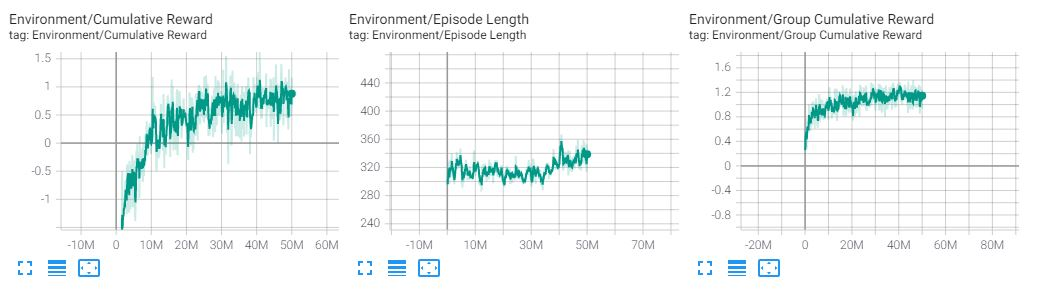
\includegraphics[width=1\textwidth]{08_Results/ML-agent results/CollaborationReward.JPG}
    \caption[Collaboration learning]{This was the optimal model for collaboration learning. The environment consisted of 2 vehicles.} \label{08:Collab}
\end{figure}